\section{Polynomial maximum depth with rank-subset scheduling}
\label{sec:polynomial-slots}

The algorithm combines exact scheduling inside a logarithmic rank cap
with the priority fallback of Section~\ref{sec:worst}. It constructs
one code for each pattern child and compares scheduling alternatives
against those codes' actual heights. In the proof, an optimal tree
certifies that at least one trial is feasible.

\subsection{The algorithm and its guarantee}

Use the count threshold $\delta$ and potential coefficient $\gamma$
of \eqref{eq:worst-parameter-conditions}. For the original input size
$n$, fix once
\begin{equation}\label{eq:global-slot-cap}
 q=\lceil\log_2n\rceil,\qquad
 R=\left\lfloor\frac{\gamma q}{\gamma-1}\right\rfloor,
 \qquad L=R+1.
\end{equation}
We fix the cap $L$ from the original size $n$ and pass it unchanged to
every recursive child; consequently, the rank-state bound stays uniform
throughout the tree. When a state contains only one hypothesis, its
identity is already known and recursion stops. At every larger state,
we first use a supplied count-balanced query whenever one is available.
Its two answer classes become the next recursive states, each with the
same cap $L$. Once no count-balanced query remains, the state is flat,
and the algorithm proceeds to the scheduling step below.

At a flat state $S$, construct every full hull-pattern child once and
record its actual height $h_A=C_W(A)$. Then try increasing integer
heights $H$ through $\lfloor(3+\gamma)(|S|-1)\rfloor$; because the
children stay fixed, each trial reuses their codes and the first passing
trial gives the smallest certified height. Compare the priority
fallback with exact adjacent-block scheduling. For the latter,
candidates are edges of the full normalized hull, with the origin kept
as a free negative marker. Each positive vertex arc therefore becomes
a circular interval of edge blocks.
Write
\[
 z_A=\lfloor\log_2(\delta |S|/|A|)\rfloor,\qquad
 B_A=\left\lfloor\frac{H-h_A-z_A-5}{2}\right\rfloor.
\]
Proposition~\ref{lem:endpoint-height} bounds the endpoint continuation
by $z_A+4$ queries after the first positive answer; the shared allowance
$z_A+5$ includes the first positive query and also covers a pinned exit.
Thus, after reserving the child height and endpoint allowance, at most
$B_A$ full blocks can precede the hit block, since each uses at most two
queries. This gives deadline $B_A+1$. The total cap
$\lfloor H/2\rfloor$ follows for the same reason: every block costs at
most two queries.
Reject negative budgets; otherwise assign block deadline $B_A+1$ and
use the total cap
\begin{equation}\label{eq:hybrid-total-cap}
 \min\{L,\lfloor H/2\rfloor\}.
\end{equation}
The scheduler receives these integer deadlines directly, so its
feasibility checks match the route-height bounds. An optional exact
whole-exit decoder, proved safe below, may be included in the same
trial. Return a passing alternative at the least height, attach its
endpoint decoders and stored child codes, and contract constant
queries. If the hull has dimension at most one, its two real extreme
tests already determine every pattern, so query them directly.

\begin{algorithm}[H]
\caption{\HybridTree: general polynomial maximum depth}
\label{alg:hybrid-tree}
\KwIn{State $S$, original size $n$, fixed global cap
$L=R+1$, where $q=\lceil\log_2 n\rceil$ and $R=\lfloor\gamma q/(\gamma-1)\rfloor$,
and the count parameters calibrated in Section~\ref{sec:worst-calibration}.}
\KwOut{A tree satisfying Theorem~\ref{thm:poly-slot-worst}.}
Stop at a singleton; at a count-balanced state query a balanced line and recurse\;
Compute $\HullData(S)$ and build each child's hybrid code once\;
Handle a low-dimensional hull directly; otherwise record child heights $h_A$\;
\For{$H=1,\ldots,\lfloor(3+\gamma)(|S|-1)\rfloor$}{
  Try $\PriorityTrial$ with these stored children\;
  Set $z_A=\lfloor\log_2(\delta|S|/|A|)\rfloor$ and
  $B_A=\lfloor(H-h_A-z_A-5)/2\rfloor$\;
  \If{all $B_A\ge0$}{
    Try circular $\SlotDP$ on full-hull-edge demands with deadlines $B_A+1$
    and slot cap $\min\{L,\lfloor H/2\rfloor\}$\;
  }
  Optionally try whole-exit $\SlotDP$ using actual endpoint-continuation
  heights and the same total cap; test feasibility with these heights\;
  \If{any alternative passes}{
    Attach its endpoint decoders and the stored child trees\;
    Terminate the negative cover at $A_0$ when present; omit that leaf otherwise\;
    \KwRet a passing tree, contracting constant queries\;
  }
}
\end{algorithm}

The global cap is inherited unchanged by every child. The priority
fallback proves that a trial always passes; the algorithm never tests
the unknown condition $\OPT_W(S)\le R$.

\begin{figure}[htbp]
\centering
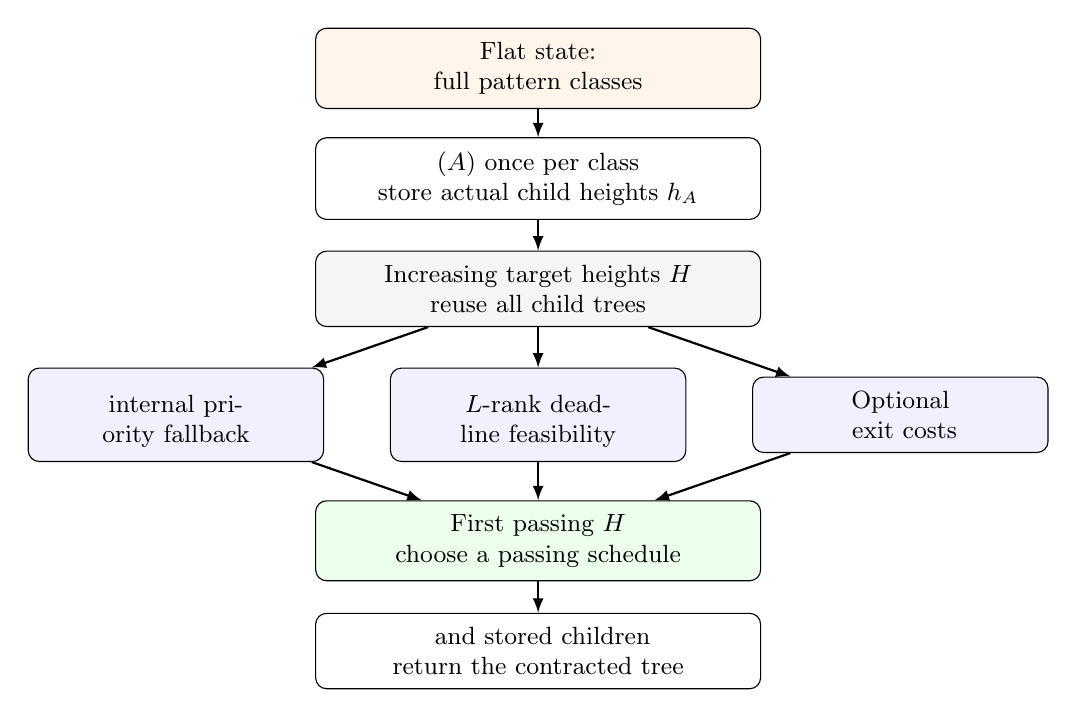
\begin{tikzpicture}[every node/.style={font=\small},
  box/.style={draw,rounded corners,align=center,inner sep=5pt,text width=3.4cm},
  wide/.style={box,text width=5.3cm},arr/.style={-latex,thick}]
  \node[wide,fill=orange!8] (hull) at (0,0)
    {Flat state: \HullData\\full pattern classes};
  \node[wide] (children) at (0,-1.4)
    {\HybridTree$(A)$ once per class\\store actual child heights $h_A$};
  \node[wide,fill=gray!8] (trial) at (0,-2.8)
    {Increasing target heights $H$\\reuse all child trees};
  \node[box,fill=blue!6] (priority) at (-4.6,-4.4)
    {\PriorityTrial\\internal priority fallback};
  \node[box,fill=blue!6] (slots) at (0,-4.4)
    {\SlotDP\\$L$-rank deadline feasibility};
  \node[box,fill=blue!6] (whole) at (4.6,-4.4)
    {Optional \SlotDP\\\EndpointCode\ exit costs};
  \node[wide,fill=green!7] (pass) at (0,-6)
    {First passing $H$\\choose a passing schedule};
  \node[wide] (attach) at (0,-7.4)
    {\EndpointCode\ and stored children\\return the contracted tree};
  \draw[arr] (hull) -- (children);
  \draw[arr] (children) -- (trial);
  \draw[arr] (trial) -- (priority);
  \draw[arr] (trial) -- (slots);
  \draw[arr] (trial) -- (whole);
  \draw[arr] (priority) -- (pass);
  \draw[arr] (slots) -- (pass);
  \draw[arr] (whole) -- (pass);
  \draw[arr] (pass) -- (attach);
\end{tikzpicture}
\caption{At a flat state, the algorithm first computes the hull and
children, then tests increasing target heights using three schedule
checks. The arrows carry the geometry, child heights, and candidate
schedules needed by those checks. The logarithmic cap $L$ is fixed at
the original root. The priority fallback guarantees a passing trial
by the stated height bound; the exact and whole-exit checks can certify
an earlier trial, and the algorithm selects the first trial accepted
by its explicit checks.}
\label{fig:hybrid-procedure-flow}
\end{figure}



\begin{theorem}[General polynomial maximum-depth approximation]
\label{thm:poly-slot-worst}
For separating supplied binary unit-cost planar line queries,
Algorithm~\ref{alg:hybrid-tree} runs in deterministic polynomial time
and returns a tree satisfying
\[
 \boxed{C_W(\HH)\le(2+\gamma)\OPT_W(\HH)<4.464966\,\OPT_W(\HH)}
\]
with the calibrated parameters of Section~\ref{sec:worst-calibration}.
A singleton has cost zero, and every query is a supplied line.
\end{theorem}

\begin{proofstrategy}
\begin{enumerate}
\item Solve interval deadlines exactly by partitioning a small set
of global query ranks (the positions assigned in the full schedule)
between spatial left and right regions.
\item Prove two recursive bounds simultaneously: the priority fallback
works for every optimum; exact scheduling improves it when the optimum
fits the global cap.
\item At the root, a small optimum uses the stronger bound. A large
optimum absorbs the fallback's count potential. Calibrate the two
count-credit inequalities only after these structural arguments.
\end{enumerate}
\end{proofstrategy}

Spatial left and right regions may be queried in an interleaved order.
The exact scheduler assigns each region a subset of global query ranks;
these positions preserve its deadlines while allowing the two searches
to interleave.

\begin{proposition}[Exact rank-subset scheduler]
\label{lem:rank-subset-scheduling}
For $N$ interval demands on $M$ ordered candidates, with integer
first-hit deadlines and at most $L$ distinct selected candidates,
feasibility and a schedule can be found in
$O(M^3 3^L+NM^2)$ time with $O(M^2 2^L)$ states.
Circular intervals add a factor $M$ by enumerating the first candidate.
\end{proposition}

The exact scheduler's short global cap makes its stronger bound
available on small-optimum states, while the priority fallback covers
the remaining states. Proving both bounds together lets the recursion
use the strongest child estimate whose threshold survives restriction.

\begin{proposition}[Two simultaneous recursive guarantees]
\label{prop:slot-invariants}
At every recursive state $S$, with $s=|S|$ and $D=\OPT_W(S)$,
\begin{align}
 C_W(S)&\le3D+\Phi(s),\label{eq:slot-universal-invariant}\\
 D\le R\quad\Longrightarrow\quad
 C_W(S)&\le2D+\Phi(s).\label{eq:slot-restricted-invariant}
\end{align}
The threshold $R$ is global, so restriction preserves the second
invariant's inductive hypothesis in every child.
\end{proposition}

A feasible abstract schedule must still account for actual endpoint
queries, stored child continuations, and the negative route. The next
statement connects those certificates to a finite legal construction.

\begin{proposition}[Executable trials and polynomial reconstruction]
\label{prop:slot-construction}
Every accepted trial has complete height at most $H$, including its
zero route when present. A passing trial is reached within the stated
range; geometry, scheduling, endpoint decoding, and reconstruction
have polynomial bit complexity. The optional whole-exit alternative
preserves both guarantees in Proposition~\ref{prop:slot-invariants}.
\end{proposition}

\begin{proof}[Proof of Theorem~\ref{thm:poly-slot-worst}]
At the root, if $D\le R$, \eqref{eq:slot-restricted-invariant} gives
$C_W\le2D+\Phi(n)\le2D+\gamma\log_2n\le(2+\gamma)D$.
The middle step removes the floor from $\Phi(n)$, while
Claim~\ref{clm:restriction-3} gives $D\ge\log_2n$; together these
facts bound the logarithmic potential by $\gamma D$.
If $D>R$, integrality gives
$D\ge R+1>\gamma q/(\gamma-1)$. Since $\log_2n\le q$,
this implies $\gamma\log_2n/D<\gamma-1$.
Substituting this bound into \eqref{eq:slot-universal-invariant} therefore gives
\[
 \frac{C_W}{D}\le3+\frac{\gamma\log_2n}{D}
 <3+(\gamma-1)=2+\gamma.
\]
Proposition~\ref{prop:slot-construction} supplies the legal
polynomial construction, and the calibration below gives its numerical
factor. Trial acceptance is determined by the constructed code; the
proof uses $D$ to show that one of the checked trials meets the bound.
\end{proof}

\subsection{Technical proofs of the propositions}

\begin{proof}[Proof of Proposition~\ref{lem:rank-subset-scheduling}]
The scheduler's state separates spatial information from temporal
information. A spatial split removes the intervals it hits; absolute
ranks preserve every deadline while allowing the left and right
searches to interleave in any order.


Candidates are $1,\ldots,M$. A demand $[a,b]$ of deadline $d$
must contain a selected candidate assigned a rank at most $d$.
For region $[l,r]$, let $\mathcal I(l,r)$ contain the original
demands wholly inside it. Define $F(l,r,T)$ for an available subset
$T\subseteq[L]$ of absolute ranks; unused ranks are allowed.
The key sufficiency question is which demands can still matter inside
a region. Interval geometry makes ancestor hits recognizable from the
region alone, while the rank subset records its remaining time slots.

\begin{claim}[Contained intervals are exactly the unhit demands]
\label{clm:slot-contained-state}
The spatial region and the absolute rank subset are sufficient state.
\end{claim}
\begin{proof}
Each region is a connected component of the candidate line after
its ancestor separator points have been deleted. An original interval
not contained in one such component must contain a deleted separator:
intervals contain every candidate between their endpoints. It was
therefore hit at an ancestor. Conversely, an interval contained in a
remaining region contains none of those separators and is unhit.
Queries in other remaining regions cannot hit it either. Thus exactly
$\mathcal I(l,r)$ remains relevant in $[l,r]$. The subset $T$ records
when its future candidates may be queried in the global order; two
regions with the same number of queries can have different available
ranks and hence different deadline feasibility.
\end{proof}
Once that state is sufficient, its earliest available rank can be used
for the next separator. Partitioning the later ranks permits every
interleaving of the left and right searches.

\begin{claim}[The earliest available rank gives an exact recurrence]
\label{clm:slot-earliest-rank}
For nonempty $\mathcal I(l,r)$ and $T$, put $t=\min T$.
Reject if a contained deadline is less than $t$; otherwise accept
precisely when some $p\in[l,r]$ and partition
$T\setminus\{t\}=T_L\mathbin{\dot\cup}T_R$ satisfy
\[
 F(l,p-1,T_L)\quad\hbox{and}\quad F(p+1,r,T_R).
\]
\end{claim}
\begin{proof}
By Claim~\ref{clm:slot-contained-state}, it suffices to check the
contained demands. For sufficiency, place $p$ at rank $t$. Every contained demand
containing $p$ is hit at rank $t$, no later than its deadline because
the preliminary test checked every contained deadline. An interval
not containing $p$ is wholly in $[l,p-1]$ or $[p+1,r]$.
The two accepted subproblems give distinct candidates with disjoint
absolute rank sets, so merging their selections by rank preserves
all their deadlines and completes the state.

For necessity, let a feasible state have first selected point $p$
at rank $t'\in T$, and put $t=\min T$. If $t<t'$, then $t$ is
unused: every other selected point has rank greater than $t'$. Assign
$p$ to $t$ and keep all other ranks fixed. If $t=t'$, leave the
schedule unchanged. Thus selected ranks remain distinct, and advancing
the first point cannot delay any first hit.
No contained deadline can be smaller than $t$, since no available
rank would then meet it. Partition the other selected ranks by
whether their candidate lies left or right of $p$, and distribute
unused ranks arbitrarily between the two parts. Each unhit interval
lies wholly on one side, so the corresponding subproblem is feasible.
This gives a partition of all $T\setminus\{t\}$ as required.
When the demand family is empty, the empty selection is feasible; a
nonempty family with $T=\varnothing$ is infeasible.
\end{proof}
The DP may leave rank gaps, which only postpone hits. Compressing
those gaps produces an executable linear schedule; choosing its first
point similarly turns a circular instance into a linear one.

\begin{claim}[Reconstruction and circular cuts preserve feasibility]
The recurrence has the stated time and state bounds.
\end{claim}
\begin{proof}
Sort selected points by their assigned ranks and remove unused slots;
all hits accelerate. Precompute existence and minimum deadline of
contained demands in $O(NM^2)$ time. There are $O(M^2 2^L)$ states,
and for a mask of size $k$ there are at most $2^{k-1}$
partitions after its minimum is removed. The coarser total bound is
\[
 \sum_{T\subseteq[L]}2^{|T|}
 =\sum_{k=0}^L\binom Lk2^k=(1+2)^L=3^L.
\]
The first equality groups masks by cardinality, and the second is
the binomial theorem. Hence all masks contribute a total partition
factor $3^L$. With $O(M^2)$ spatial regions and at most $M$ candidate
roots per region, the transitions take $O(M^3 3^L)$ time, in addition
to the $O(NM^2)$ preprocessing. Removing unused ranks sends every
assigned rank to an earlier or equal schedule position, so no deadline
is missed.

An empty circular demand family accepts immediately. Otherwise
enumerate its first selected point at rank one. Delete the intervals
hit there and cut the candidate circle at that point; every survivor
becomes an ordinary interval. A surviving original deadline at most
one is impossible. For all other survivors subtract one from their
deadline and use $L-1$ remaining slots. Appending the first point
to any accepted linear schedule restores the original deadlines,
and every feasible circular schedule has one of the enumerated first
points. The enumeration adds a factor $M$.
\end{proof}
\end{proof}

Within an interval state, the earliest available rank must be assigned
to one candidate $p$. Choosing $p$ divides the remaining candidates
into left and right intervals, and the unused ranks must split between
those two subproblems. The recursion enumerates these partitions;
memoization reuses each interval-and-rank state.

\begin{algorithm}[H]
\caption{\SlotDP: exact interval deadlines with a rank subset}
\label{alg:slot-dp}
\KwIn{Ordinary interval demands and deadlines; region $[l,r]$;
available absolute ranks $T\subseteq[L]$.}
\KwOut{A feasible rank assignment, or infeasible.}
\If{no original demand is wholly contained in $[l,r]$}{\KwRet the empty assignment\;}
\If{$T=\varnothing$}{\KwRet infeasible\;}
\If{this state is memoized}{\KwRet its stored result\;}
$t\gets\min T$\;
\If{a wholly contained demand has deadline $<t$}{\KwRet infeasible\;}
\ForEach{$p\in[l,r]$ and $T_L\subseteq T\setminus\{t\}$}{
  $T_R\gets T\setminus(T_L\cup\{t\})$\;
  Recurse on $([l,p-1],T_L)$ and $([p+1,r],T_R)$\;
  \If{both assignments are feasible}{
    Memoize their union with $(p,t)$ and \KwRet it\;
  }
}
Memoize and return infeasible\;
\end{algorithm}

After the recursion succeeds, sort the selected candidates by rank and
suppress unused ranks to obtain the schedule. For circular demands,
enumerate the first candidate and cut the circle there; this converts
the remaining demands to intervals, with one subtracted from their
deadlines and the slot cap to account for the forced first rank.
In the optional complete-exit variant, first compute both oriented
decoder costs using Algorithm~\ref{alg:endpoint-code}. Those costs
replace the ordinary deadline precheck by the local height tests of
Section~\ref{sec:polynomial-slots}; the same rank partitions then
handle the remaining scheduling choices.


\begin{proof}[Proof of Proposition~\ref{prop:slot-invariants}]
Induct on $s$, with zero-cost singleton states, proving both bounds
simultaneously. A balanced child $A$ has $\OPT_W(A)\le D$ and
$\Phi(|A|)\le\Phi(s)-1$, by restriction and
Proposition~\ref{lem:worst-floor-credit}. For either coefficient
$c\in\{2,3\}$, its inductive route bound gives
\[
 1+h_A\le1+c\OPT_W(A)+\Phi(|A|)
          \le cD+\Phi(s).
\]
The first inequality is the appropriate inductive hypothesis; in the
second, restriction bounds the optimal child height by $D$ and the
unit potential drop pays for the root query.
When $c=2$, $D\le R$ also gives $\OPT_W(A)\le R$, so the
stronger child hypothesis is available. Thus a balanced query
preserves either bound. The priority alternative
preserves the universal bound by Proposition~\ref{thm:worst}; smaller
actual children only improve its budgets.

For the stronger flat-state bound, assume $D\le R$ and put
$H^*=2D+\Phi(s)$. All children meet the same global threshold, so
their stronger inductive bound is available.
The stronger flat-state proof has three parts: convert child-height
credit into deadlines, fit a comparison cover inside both caps, and
translate its blocks into physical routes. The optimal witness is used
only to establish existence of a passing trial.

\begin{claim}[Actual child heights give feasible comparison deadlines]
\label{clm:slot-child-deadlines}
Every nonzero class satisfies $B_A+1\ge t_A$ at $H^*$.
\end{claim}
\begin{proof}
Proposition~\ref{lem:height-prefix} gives $\OPT_W(A)\le D-(t_A-1)$.
The actual stored height therefore satisfies
$h_A\le2[D-(t_A-1)]+\Phi(|A|)$. Substitution gives
\begin{align*}
 H^*-h_A-z_A-5
 &\ge2(t_A-1)+\Phi(s)-\Phi(|A|)-z_A-5\\
 &\ge2(t_A-1),
\end{align*}
The first inequality substitutes the stronger inductive child bound;
the second uses the nonzero-class count credit of
Proposition~\ref{lem:worst-floor-credit}, namely
$\Phi(s)-\Phi(|A|)\ge z_A+5$. Thus
\begin{equation}\label{eq:slot-deadline-credit}
 H^*-h_A-z_A-5\ge2(t_A-1).
\end{equation}
Dividing by two gives a lower bound by the integer $t_A-1$;
taking a floor consequently preserves it, so $B_A\ge t_A-1\ge0$.
Thus this comparison trial passes the nonnegative-budget check and has
deadline $B_A+1\ge t_A$.
This links an unknown optimal witness to deadlines computed from
actual stored codes.
\end{proof}
The comparison must satisfy each block deadline, the global rank cap,
and the cap on the negative route. A terminal nonzero singleton may
require one appended block, which accounts for the extra slot in the
global cap.

\begin{claim}[The comparison fits both total caps]
\label{clm:slot-total-caps}
Every class meets its deadline in a cover of at most $D+1$ edge blocks.
\end{claim}
\begin{proof}
Map each witness-path query to a full-hull edge containing its
supports. Enlarging a singleton support only accelerates hits; delete
repeated and unproductive blocks. If the path ends at an uncovered
nonzero singleton, append an incident edge at its supporting index
$r+1$, with $r\le D$. If the zero class exists it is the terminal
witness leaf and no append is needed. The comparison has at most $D$
blocks with a zero class and at most $D+1$ otherwise, and it hits
$A$ by rank $t_A$. Since $D\le R$, this fits $L=R+1$.
Also $s\ge2$ gives $\log_2s\ge1$, and $\gamma>2$ gives
$\Phi(s)=\lfloor\gamma\log_2s\rfloor\ge2$. As $D$ is
an integer,
\[
 \left\lfloor\frac{H^*}{2}\right\rfloor
 =\left\lfloor D+\frac{\Phi(s)}2\right\rfloor
 =D+\left\lfloor\frac{\Phi(s)}2\right\rfloor\ge D+1.
\]
Pulling the integer $D$ through the floor gives the second equality,
and $\Phi(s)\ge2$ gives the final inequality.
Thus the comparison fits both the $L$-block rank limit and the cap
$2\lfloor H^*/2\rfloor$ on the all-negative route, even when a
terminal singleton block has been appended.
\end{proof}
An abstract edge block becomes at most two supplied queries. The
second first-positive exit has a cached negative neighbor and a cheaper
decoder; accounting for this asymmetry yields one safe block allowance.

\begin{claim}[A feasible block trial bounds every physical route]
\label{clm:slot-physical-route}
Class $A$ first hit at block $k$ has complete route height at most
\begin{equation}\label{eq:slot-block-allowance}
 2(k-1)+z_A+5+h_A.
\end{equation}
\end{claim}
\begin{proof}
The preceding $k-1$ blocks use at most $2(k-1)$ supplied queries.
If the first endpoint of block $k$ is positive, discovery uses at
most $2k-1$ queries. Proposition~\ref{lem:endpoint-height} then
adds its $z_A+4$ endpoint allowance and the stored height $h_A$, so
the complete route is bounded by
\[
 (2k-1)+(z_A+4)+h_A=2(k-1)+z_A+5+h_A.
\]
If the second endpoint gives the first positive answer, the first
endpoint is a cached negative neighbor. The pinned allowance in
Proposition~\ref{lem:endpoint-height} therefore gives
\[
 2k+(z_A+2)+h_A=2(k-1)+z_A+4+h_A,
\]
which is one query smaller than the stated common allowance.
A block with one real endpoint obeys the first bound; cached answers
and the origin marker cost nothing. Put $X=H^*-h_A-z_A-5$.
Since $B_A=\lfloor X/2\rfloor$ and $k-1\le B_A$,
\[
 2(k-1)+z_A+5+h_A
 \le2\lfloor X/2\rfloor+z_A+5+h_A
 \le X+z_A+5+h_A=H^*.
\]
The last inequality is $2\lfloor X/2\rfloor\le X$.
Thus either positive route fits the trial. The all-negative route has at most
$2\lfloor H^*/2\rfloor\le H^*$ queries and identifies $A_0$ if
present; an absent zero leaf is omitted.
\end{proof}
Claims~\ref{clm:slot-child-deadlines} and~\ref{clm:slot-total-caps}
provide a feasible comparison schedule. Hence
Proposition~\ref{lem:rank-subset-scheduling} finds a passing trial at
$H^*$, and Claim~\ref{clm:slot-physical-route} converts it into the
required route-height bound.
If the hull has dimension at most one, its at most two extreme tests
learn the pattern directly. For a nonzero class the stronger child
bound and Proposition~\ref{lem:worst-floor-credit} give
$2+h_A\le2D+\Phi(s)-z_A-3\le H^*$, since $z_A\ge0$.
The all-negative route also uses at most two tests, and $H^*\ge2$.
The universal calculation is identical with coefficient three.
Both invariants follow by induction.
\end{proof}

\begin{proof}[Proof of Proposition~\ref{prop:slot-construction}]
The local route certificate and \eqref{eq:slot-block-allowance} prove
the accepted-height tests. The universal invariant supplies a passing
integer trial. Indeed $D\le s-1$ follows from a proper identifying
tree, and $\log_2s\le s-1$ for integer $s\ge1$, so
\[
 3D+\Phi(s)
 \le3(s-1)+\lfloor\gamma(s-1)\rfloor
 =\lfloor(3+\gamma)(s-1)\rfloor,
\]
where the equality uses the integrality of $3(s-1)$.
The remaining obligations are running time and reconstruction. The
rank search is exponential only in the cap fixed at the root, while
all recursive stages retain explicit supplied queries and child codes.

\begin{claim}[The global cap makes exact scheduling polynomial]
All arithmetic and the complete reconstructed tree have polynomial size.
\end{claim}
\begin{proof}
For fixed $\gamma$, put $\alpha=\gamma/(\gamma-1)$.
For $n\ge2$, $q=\lceil\log_2n\rceil<\log_2n+1$ and
$L=\lfloor\alpha q\rfloor+1<\alpha\log_2n+\alpha+1$.
For either $b=2$ or $b=3$, exponentiating gives
\[
 b^L<b^{\alpha+1}b^{\alpha\log_2n}
     =b^{\alpha+1}n^{\alpha\log_2b}.
\]
The inequality uses monotonicity of $b^x$ for $b>1$, and the
equality follows from $b^{\log_2n}=n^{\log_2b}$.
The constants are fixed, so both rank-mask costs are polynomial.
The singleton input returns immediately. There are polynomially many
trial heights and first blocks, and at most $n-1$ nonterminal
recursive stages with disjoint child sets. To see this count, the
recursive states form a rooted partition tree whose leaves are
individual hypotheses. Each nonterminal state has at least two
nonempty children: balanced queries split properly, and a flat
nonsingleton state cannot be one class because every nonzero class
has size less than $\delta s$ and the zero class has size at most
one. In a rooted tree with $n$ leaves and at least two children at
each internal vertex, counting edges gives at most $n-1$ internal
vertices. The witness LP, hull
incidence, and endpoint codes have polynomial bit complexity.
Every recursive child is smaller: balanced queries split properly,
nonzero patterns have size below $\delta s$, and $A_0$ is a singleton.
Compute $q$ and $z_A$ from their defining power-of-two thresholds, then
set $R=\lfloor\gamma q/(\gamma-1)\rfloor$. Priority weights
have $O(n\log n)$ bits. Contracting constant queries gives a proper
tree with at most $n$ leaves and $n-1$ internal nodes.
\end{proof}
Fixed endpoint allowances make the deadline instance simple, but may
overestimate a particular exit. An exact rectangle decoder can inspect
the realized patterns and their stored continuations. It uses the same
legal endpoint comparisons and therefore can only improve a trial.

\begin{claim}[Exact whole-exit decoding cannot weaken a trial]
The optional alternative is polynomial under the same cap and
accepts every fixed-allowance schedule.
\end{claim}
\begin{proofstrategy}
\begin{enumerate}
\item Use dynamic programming on endpoint-coordinate rectangles, and
      prove by induction on the realized classes that the recurrence
      gives the minimum continuation height.
\item Show that unhit interval demands are exactly those contained in
      the current region. This makes each rectangle decoder independent
      of queries already resolved outside it.
\item Compare the minimizing decoder with the explicit endpoint code
      used by a fixed-allowance schedule; its route bounds imply that the
      same schedule passes the more precise height test.
\item Count the rectangles and threshold transitions, then include the
      rank-subset factor $3^L$.
\end{enumerate}
\end{proofstrategy}
\begin{proof}
After the legal cut, each class has one realized endpoint pair; let
$M$ be the number of hull candidate positions.
For a coordinate rectangle $U$, give a one-class leaf value $h_A$
and compute
\[
 E(U)=\min_{\text{proper supplied coordinate thresholds }\ell}
 \bigl(1+\max\{E(U\cap\ell^-),E(U\cap\ell^+)\}\bigr),
\]
ignoring empty outcomes. For an empty rectangle no decoder is
needed. A rectangle containing only class $A$ has value $h_A$;
otherwise two distinct endpoint pairs differ in some coordinate,
and a legal hull comparison between those coordinate values gives
a proper threshold. Each proper threshold sends its realized pairs
to strictly smaller nonempty sets. Induction on the number of realized pairs
shows exactness: every permissible endpoint tree has such a first
threshold and costs one plus the larger continuation height, while
attaching the two minimizing continuations attains that value.
A rectangle is specified by two boundaries in each coordinate,
giving $O(M^4)$ rectangles, with $O(M)$ thresholds to try in each.
The leaf values include the stored class continuations. A pinned
endpoint is the same recurrence in one coordinate.

At state $([l,r],T)$, Claim~\ref{clm:slot-contained-state} identifies
the unhit demands as precisely the original intervals contained in
$[l,r]$. For candidate block $p$ in either
orientation, compute the whole decoder heights $E_1(l,r,p)$ and
$E_2(l,r,p)$ for its first-positive and second-first-positive cells.
These cells depend only on the region and block: an outside query
cannot hit a contained interval, and a crossing interval was already
hit by an ancestor. At $k=\min T$, replace the fixed-deadline check by
\[
 2(k-1)+1+E_1(l,r,p)\le H,\qquad 2k+E_2(l,r,p)\le H,
\]
omitting empty cells. Keep the rank partitions, circular first-block
enumeration, and negative-route cap. These prefixes conservatively
include cached endpoints and the origin. For a cell containing classes $A$, the explicit endpoint code with
their stored continuations is a feasible rectangle decoder tree. Its
whole height is at most $\max_A(e_A^{(4)}+h_A)$ on a first-positive
cell and at most $\max_A(e_A^{(2)}+h_A)$ on a pinned cell.
Therefore the minimizing values $E_1,E_2$ are no larger than these
bounds. If each fixed-allowance class route passes at block rank $k$,
then respectively
$2(k-1)+1+E_1\le H$ and $2k+E_2\le H$.
Keeping the same candidate schedule and negative-route cap thus
passes the whole-exit trial as well. Precomputation and the rank-subset
transitions are polynomial times $3^L$.
\end{proof}
\end{proof}

\subsection{Parameter calibration}
\label{sec:worst-calibration}

\begin{parameterchoice}
The balanced-query and flat-decoder credits require
\[
 \gamma(\delta)=\max\left\{
 \frac1{\log_2(1/(1-\delta))},\,
 \frac5{\log_2(1/\delta)}\right\}.
\]
The first term decreases with $\delta$, while the second increases,
so their maximum is minimized where they meet. Equating them gives
$\delta=(1-\delta)^5$. Let $\delta_0$ be the
unique root of this equation in $(0,1/3)$, and set
\[
 \gamma_0=\frac1{\log_2(1/(1-\delta_0))}
         =\frac5{\log_2(1/\delta_0)}.
\]
In the algorithm, take $\delta=\delta_0$ and $\gamma=\gamma_0$.
The root is unique because $x-(1-x)^5$ is strictly increasing on this
interval: its first term increases and its second decreases. Its values
at $0$ and $1/3$ are $-1$ and $49/243$, respectively, so it crosses
zero once. Thus
$\gamma_0\log_2(1/(1-\delta_0))=1$ and
$\gamma_0\log_2(1/\delta_0)=5$, so both count-credit conditions hold
at equality. To bound the resulting factor,
put $a=245122333/10^9$ and $b=245122334/10^9$. Exact substitution gives
$a-(1-a)^5<0<b-(1-b)^5$, so $a<\delta_0<b$. The first function in
$\gamma(\delta)$ is decreasing and the second is increasing; hence
\[
 \gamma_0\le\frac1{\log_2(1/(1-a))},\qquad
 \gamma_0\le\frac5{\log_2(1/b)}.
\]
Applying the rational logarithm enclosure
\eqref{eq:rational-log-bounds} with $N=100$ to these endpoint
expressions certifies that both upper bounds are less than
$G=2464966/10^6$. More explicitly, if $U_{100}(2)$ is the upper
endpoint for $\ln2$ in that enclosure, the exact rational comparisons
are
\[
 \frac{L_{100}(1/(1-a))}{U_{100}(2)}>\frac{10^6}{2464966},
 \qquad
 \frac{L_{100}(1/b)}{U_{100}(2)}>\frac{5\cdot10^6}{2464966}.
\]
Each numerator is the lower endpoint for its logarithm, so these
comparisons imply the claimed upper bounds on $\gamma_0$. Also
$\delta_0<b<1/4$, so
$1/(1-\delta_0)<4/3<\sqrt2$ (since $16/9<2$) and therefore
$\gamma_0>2$. Thus
\[
 \boxed{2+\gamma_0<4.464966.}
\]
\end{parameterchoice}

The same calibration gives
$\alpha=\gamma/(\gamma-1)$.
Since $q<\log_2n+1$, the rank-mask contributions obey
\[
 3^L<3^{\alpha+1}n^{\alpha\log_2 3},\qquad
 2^L<2^{\alpha+1}n^\alpha,
\]
Thus each is polynomial in $n$, as required for the scheduling
component. The full algorithm's exponent also includes its other stages.
The ceiling $q=\lceil\log_2 n\rceil$ is found by comparing integer
powers of two with $n$.

